%
\documentclass{article}
\usepackage{amsmath,amssymb,bbm,amsthm}
\usepackage{fullpage}
\usepackage{thm-restate,color,xcolor,xspace}
\usepackage{hyperref,cleveref}
\usepackage{thmtools}
\usepackage{graphicx}
\usepackage{algorithm,algorithmic}



\newtheorem{theorem}{Theorem}
\newtheorem{lemma}[theorem]{Lemma}
\newtheorem{definition}[theorem]{Definition}
\newtheorem{corollary}[theorem]{Corollary}
\newtheorem{observation}[theorem]{Observation}
\newtheorem{claim}[theorem]{Claim}
\newtheorem{subclaim}{Subclaim}
\newtheorem{fact}[theorem]{Fact}
\newtheorem{assumption}[theorem]{Assumption}
\newtheorem{remark}[theorem]{Remark}

\def\BAL#1\EAL{\begin{align*}#1\end{align*}}
\def\BALN#1\EALN{\begin{align}#1\end{align}}
\def\BG#1\EG{\begin{gather}#1\end{gather}}
\newcommand{\na}{\nabla}
\newcommand{\ang}[1]{\left\langle#1\right\rangle}

\begin{document}


\title{convex notes}
\date{\today}
\maketitle

\section{Gradient descent}

\begin{definition}[$\beta$-smooth]
A function $f$ is $(\beta,q)$-smooth if the gradient $\na f$ is $\beta$-Lipschitz in the dual norm:
\BG
\left\lVert\na f(x)-\na f(y)\right\rVert \le \beta\left\lVert x-y\right\rVert .\label{eq:smooth1}
\EG
\end{definition}

\begin{lemma}[(\ref{eq:smooth1})$\implies$(\ref{eq:smooth2})]
Let $f$ be a $\beta$-smooth function on $\mathbb R^n$. Then, for any $x,y\in\mathbb R^n$,
\BG
f(x)-f(y)-\na f(y)^T(x-y)  \le \frac\beta2\left\lVert x-y\right\rVert^2 . \label{eq:smooth2}
\EG
\end{lemma}
\begin{proof}
We first represent $f(x)-f(y)$ as an integral. Let $g(t)=f(y+t(x-y))$, so that $g'(t)=\na f(y+t(x-y))^T(x-y)$, since it's the rate of change of $f$ at point $y+t(x-y)$ in the direction $x-y$. By fundamental theorem of calculus,
\[ f(x)-f(y)=g(1)-g(0)=\int_0^1g'(t)dt=\int_0^1\na f(y+t(x-y))^T(x-y)  dt .\]
We apply Cauchy-Schwarz and then $\beta$-smoothness:
\BAL
f(x)-f(y)-\na f(y)^T(x-y) &= \int_0^1\na f(y+t(x-y))^T(x-y)dt - \na f(y)^T(x-y) 
\\&= \int_0^1\big( \na f(y+t(x-y))-\na f(y)\big)^T(x-y)dt
\\&\le\int_0^1\left\lVert\na f(y+t(x-y))-\na f(y)\right\rVert\cdot\left\lVert x-y\right\rVert dt
\\&\le\int_0^1\beta t\left\lVert x-y\right\rVert^2dt
\\&=\frac\beta2\left\lVert x-y\right\rVert^2 .
\EAL
\end{proof}
Therefore, if $f$ is both convex and $\beta$-smooth, then
\BG
0\le f(x)-f(y)-\na f(y)^T(x-y)  \le \frac\beta2\left\lVert x-y\right\rVert^2 .
\EG

In fact, \Cref{eq:smooth1,eq:smooth2} are equivalent for convex functions, so we could have defined $\beta$-smooth using either equation.
\begin{lemma}[(\ref{eq:smooth2})$\implies$(\ref{eq:smooth1})]
Let $f$ be a convex function satisfying (\ref{eq:smooth2}). Then, $f$ is $\beta$-smooth.
\end{lemma}
\begin{proof}
Let 
\[ z=y-\frac1\beta(\na f(y)-\na f(x)) .\]
Then,
\BAL
f(x)-f(y)&=f(x)-f(z)+f(z)-f(y)
\\&\stackrel{\text{convex},(\ref{eq:smooth2})}\le\na f(x)^T(x-z)+\na f(y)^T(z-y)+\frac\beta2\left\lVert z-y\right\rVert^2
\\&=\na f(x)^T(x-y)+(\na f(x)-\na f(y))^T(y-z)+\frac1{2\beta}\left\lVert\na f(x)-\na f(y)\right\rVert^2
\\&=\na f(x)^T(x-y)+(\na f(x)-\na f(y))^T\left(\frac1\beta(\na f(y)-\na f(x))\right)+\frac1{2\beta}\left\lVert\na f(x)-\na f(y)\right\rVert^2
\\&=\na f(x)^T(x-y)-\frac1{2\beta}\left\lVert\na f(x)-\na f(y)\right\rVert^2 .
\EAL
Rearranging,
\BAL
\frac1{2\beta}\left\lVert\na f(x)-\na f(y)\right\rVert^2 \le f(y)-f(x)-\na f(x)^T(y-x) \stackrel{(\ref{eq:smooth2})}\le \frac\beta2\left\lVert x-y\right\rVert^2.
\EAL
Taking the square root finishes the proof.
\end{proof}

Consider a gradient step $y=x-\frac1\beta\na f(x)$. From (\ref{eq:smooth2}), we get
\[ f\left( x-\frac1\beta\na f(x)\right)-f(x)+\na f(x)^T\left(\frac1\beta\na f(x)\right) = f(y)-f(x)-\na f(x)^T(y-x) \le \frac\beta2\left\lVert x-y\right\rVert^2 = \frac\beta2\left\lVert\frac1\beta\na f(x)\right\rVert^2 \]
\BG
\iff f\left( x-\frac1\beta\na f(x)\right)-f(x)\le-\frac1{2\beta}\left\lVert\na f(x)\right\rVert^2 .\label{eq:gd-step}
\EG
Basically, the step size $\eta=\frac1\beta$ is chosen small enough that the linear (in the step size) term $-\na f(x)^T(y-x)$ dominates the quadratic term $\frac\beta2\left\lVert\frac1\beta\na f(x)\right\rVert^2$.

\begin{theorem}
Let $f$ be convex and $\beta$-smooth. Then, gradient descent with $\eta=\frac1\beta$ satisfies
\[ f(x_t)-f(x^*)\le\frac{2\beta\left\lVert x_1-x^*\right\rVert^2}{t-1} .\]
\end{theorem}
\begin{proof}
By (\ref{eq:gd-step}), we have
\[ f(x_{x+1})-f(x_s)\le-\frac1{2\beta}\left\lVert\na f(x_s)\right\rVert^2 .\]
Let $\delta_s=f(x_s)-f(x^*)$ be how close the current point is to optimal. Rewriting,
\[ \delta_{s+1}\le\delta_s-\frac1{2\beta}\left\lVert\na f(x_s)\right\rVert^2 .\]
Also, by convexity,
\[ \delta_{s+1}=f(x_s)-f(x^*)\le\na f(x_s)^T(x_s-x^*)\le\left\lVert x_s-x^*\right\rVert\cdot\left\lVert\na f(x_s)\right\rVert ,\]
which, intuitively, means that $\na f(x_s)$ should decrease at least as much as if the function were a straight line between $x_s$ and $x^*$ (because $f$ is convex).
We will prove that $\left\lVert x_s-x^*\right\rVert$ is decreasing with $s$; assuming this, we obtain
\[ \delta_{s+1} \le \left\lVert x_s-x^*\right\rVert\cdot\left\lVert\na f(x_s)\right\rVert \le \left\lVert x_1-x^*\right\rVert\cdot\left\lVert\na f(x_s)\right\rVert \]
\[ \implies \delta_{s+1}\le\delta_s-\frac1{2\beta}\left\lVert\na f(x_s)\right\rVert^2 \le \delta_s-\frac1{2\beta}\left(\frac{\delta_{s+1}}{\left\lVert x_1-x^*\right\rVert}\right)^2=\delta_s-\frac1{2\beta\left\lVert x_1-x^*\right\rVert^2}\delta_s^2 . \]
To finish the theorem, iterate and prove by induction.

To show that $\left\lVert x_s-x^*\right\rVert$ decreases, we use (\ref{eq:smooth2}) twice, with $x$ and $y$ exchanged, to obtain
\[ (\na f(x)-\na f(y))^T(x-y) \ge \frac1\beta\left\lVert\na f(x)-\na f(y)\right\rVert^2 .\]
Plugging in $x\gets x_s$ and $y\gets x^*$ and using that $\na f(x^*)=0$, 
\[ \na f(x_s)^T(x_s-x^*)\ge\frac1\beta\left\lVert\na f(x)\right\rVert^2 .\]
Therefore,
\BAL
\left\lVert x_{s+1}-x^*\right\rVert^2=\left\lVert x_s-\frac1\beta\na f(x_s)-x^*\right\rVert^2
&=\left\lVert x_s-x^*\right\rVert^2-\frac2\beta\na f(x_s)^T(x_s-x^*)+\frac1{\beta^2}\left\lVert\na f(x_s)\right\rVert^2
\\&\le\left\lVert x_s-x^*\right\rVert^2-\frac2{\beta^2}\left\lVert\na f(x_s)\right\rVert^2+\frac1{\beta^2}\left\lVert\na f(x_s)\right\rVert^2
\\&=\left\lVert x_s-x^*\right\rVert^2-\frac1{\beta^2}\left\lVert\na f(x_s)\right\rVert^2
\\&\le\left\lVert x_s-x^*\right\rVert^2.
\EAL
\end{proof}

\section{Mirror descent}

\begin{definition}[Bregman divergence]
$V_x^r(y) = r(y) - r(x) - \langle\nabla r(x), y-x\rangle$
\end{definition}

\begin{lemma}[Three-point equality]
$V_x^r(y) + V_y^r(z) = V_x^r(z) + \langle\nabla r(x)-\nabla r(y), z-y\rangle$
\end{lemma}
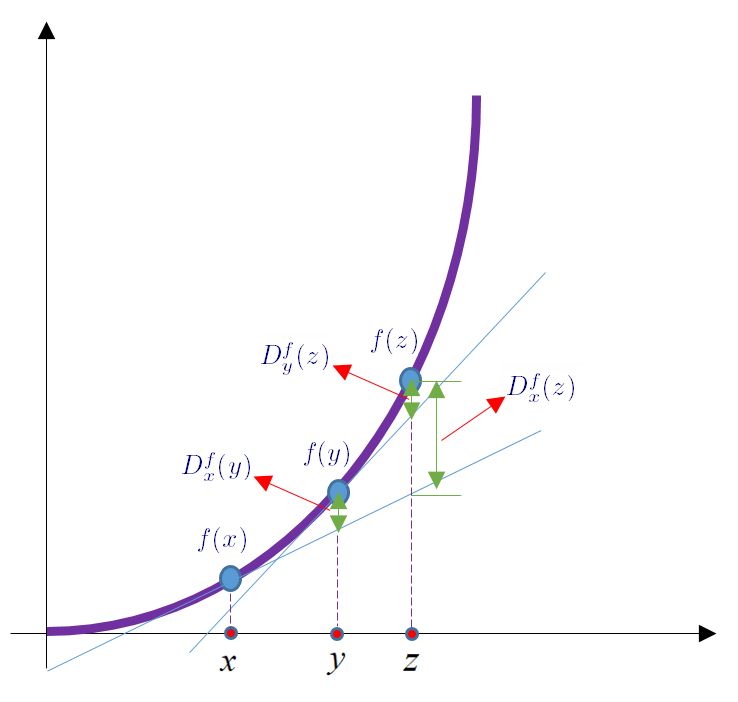
\includegraphics[scale=.5]{three-point.png}
\begin{proof}
Expanding the Bregman divergence terms, the $r(x),r(y),r(z)$ terms match. For the inner product terms, we have $-\langle\nabla r(x),y-x\rangle-\langle\nabla r(y),z-y\rangle$ on the left and $-\langle\nabla r(x),z-x\rangle + \langle\nabla r(x)-\nabla r(y),z-y\rangle$ on the right. These terms clearly match up.
\end{proof}

\begin{lemma}[Three-point inequality]
Let $f$ be a smooth function and let $y=\arg\min\{\langle\nabla f(x),y\rangle+ V_x^r(y)\}$. Then, for any $z$ in the (convex) domain,
\[ \langle\nabla f(x), y-z\rangle \le V_x^r(z) - V_x^r(y) - V_y^r(z) \]
\end{lemma}
\begin{proof}
Re-arranging the three-point equality,
\[  \langle\nabla r(x)-\nabla r(y), y-z\rangle = V_x^r(z) - V_x^r(y) - V_y^r(z) . \]
It remains to show that
\[ \langle\nabla f(x)-\nabla r(x)+\nabla r(y), y-z\rangle \le 0 .\]
Suppose first that the domain is everything. Then, the minimizer $y$ satisfies
\[ 0 = \nabla_y(\langle\nabla f(x),y\rangle+ V_x^r(y)) = \nabla_y\big(\langle\nabla f(x),y\rangle+r(y)-r(x)-\langle\nabla r(x),y-x\rangle\big) = \nabla f(x) + \nabla r(y) - \nabla r(x) ,\]
so the inequality above is actually an equality. More generally, we must have $\langle\nabla f(x) + \nabla r(y) - \nabla r(x), z-y\rangle\ge0$ since moving the solution from the minimizer $y$ in the direction of $z$ can only increase the function value.
\end{proof}

\paragraph{Mirror descent.}
Start with an arbitrary $x_0$. For each iteration $t\in[T]$, let $x_{t+1}=\arg\min\{\langle\nabla f(x_t),y\rangle+V_{x_t}^r(y)\}$.

\begin{lemma}
Assume that
 \begin{enumerate}
 \item $V_x^r(y)$ is $1$-strongly convex for all $x,y$ in the primal norm: $V_x^r(y)\ge\frac12\left\lVert x-y\right\rVert^2$
 \item $V_x^r(y) \le R$ for all $x,y$ in the domain
 \item $\left\lVert\nabla f(x)\right\rVert_*\le L$ for all $x$ in the domain.
 \end{enumerate}
Then, running mirror descent for $T$ iterations gives
\[ \sum_{t=0}^{T-1}\langle\nabla f(x_t), x_t-x^*\rangle \le R+ \frac{L^2T}2 .\]
\end{lemma}
\begin{proof}
By the three-point inequality,
\[ \langle\nabla f(x_t), x_{t+1}-x^*\rangle \le V_{x_t}^r(x^*) - V_{x_t}^r(x_{t+1}) - V_{x_{t+1}}^r(x^*) \le V_{x_t}^r(x^*) - \frac12\left\lVert x_t-x_{t+1}\right\rVert^2 - V_{x_{t+1}}^r(x^*)  . \]
Adding $\langle\nabla f(x_t),x_t-x_{t+1}\rangle$ to both sides, and then applying Cauchy-Schwarz and then AM-GM on
\[ \langle\nabla f(x_t),x_t-x_{t+1}\rangle \le \left\lVert\nabla f(x_t)\right\rVert_* \cdot \left\lVert x_t-x_{t+1}\right\rVert \le \frac12\left\lVert\nabla f(x_t)\right\rVert_*^2 + \frac12\left\lVert x_t-x_{t+1}\right\rVert^2 ,\]
we obtain
\[ \langle\nabla f(x_t), x_t-x^*\rangle \le V_{x_t}^r(x^*)-V_{x_{t+1}}^r(x^*) + \frac12\left\lVert\nabla f(x_t)\right\rVert_*^2 \le V_{x_t}^r(x^*)-V_{x_{t+1}}^r(x^*) + \frac{L^2}2 .\]
Summing over all $t\in[0,T-1]$, the terms $V_{x_t}^r(x^*)-V_{x_{t+1}}^r(x^*)$ telescope, and we obtain
\[ \sum_{t=0}^{T-1}\langle\nabla f(x_t), x_t-x^*\rangle \le V_{x_0}^r(x^*)-V_{x_T}^r(x^*) + \frac{L^2T}2 .\]
The lemma follows from $0 \le V_x^r(y)\le R$ for all $x,y$ by assumption.
\end{proof}
Suppose that we instead set $x_{t+1}=\arg\min\{\langle\eta\nabla f(x_t),y\rangle+V_{x_t}^r(y)\}$ for some parameter $\eta>0$. We can essentially replace $f(x)$ with $\eta f(x)$ in the lemma above, which gives the guarantee
\[ \eta \sum_{t=0}^{T-1}\langle\nabla f(x_t), x_t-x^*\rangle \le R + \frac{(\eta L)^2T}2 .\]
The average regret is $\frac1{\eta T}(R+\eta^2L^2T/2) = R/(\eta T) + \eta L^2/2$, and optimizing $\eta$ gives $O(\sqrt{RL^2/T})$, which is decreasing in $T$. Finally, setting $T=O(RL^2/\epsilon^2)$ gives average regret $\epsilon$. Note that this coincides with multiplicative weights intuition: the dependency on $\epsilon$ is $1/\epsilon^2$, the dependency on the diameter $R$ is linear (usually $O(\log n)$ for multiplicative weights), and the dependency on the width $L$ is quadratic.

\section{old mirror descent notes}

Define the Bregman divergence 
\[ D_f(x,y) := f(x) - f(y) - \langle\nabla f(y), x-y\rangle ,\]
which is always nonnegative when $f$ is convex.

Mirror descent begins with $x_0$ arbitrarily, and then sets
 \begin{itemize}
 \item $y_i\gets\nabla f(x_i)$ (mirror map to dual)
 \item $y_{i+1}\gets y_i-\eta\nabla f(x_i)$ (take gradient step in dual)
 \item $x_{i+1}\gets\nabla f^*(y_{i+1})$, i.e., select $x_{i+1}$ s.t.\ $y_{i+1}=\nabla f(x_{i+1})$ (mirror map back)
% \im $x_{i+1}\gets\min_{x\in\m D}D_f(x,x'_{i+1})$ (projection)
 \end{itemize}
Let $\overline x:=\frac1T\sum_{i=0}^{T-1}x_i$ be the average. We want to show that
\[ f(\overline x)-f(x)\stackrel!\le\epsilon. \]
We begin with
\[ f(\overline x) = f\left(\frac1T\sum_{i=0}^{T-1}x_i\right) \le \frac1T\sum_{i=0}^{T-1}f(x_i),\]
so
\[ f(\overline x) -f(x)\le \frac1T\sum_{i=0}^{T-1}f(x_i)-f(x)\le \frac1T\sum_{i=0}^{T-1}\big(f(x_i)-f(x)\big)\le\frac1T\sum_{i=0}^{T-1}\langle\nabla f(x_i), x_i-x\rangle .\]
To see the last inequality, simply flip the sign of the convexity inequality $f(x)-f(x_i)\ge\langle\nabla f(x_i),x-x_i\rangle$.

Since the gradient steps in the dual are $\eta\nabla f(x_i)$, we can rewrite it as
\[ f(\overline x)-f(x) \le\frac1T\sum_{i=0}^{T-1}\langle\nabla f(x_i), x_i-x\rangle = \frac1T\sum_{i=0}^{T-1}\langle \frac1\eta(y_i-y_{i+1}), x_i-x\rangle  \frac1T\sum_{i=0}^{T-1}\langle \frac1\eta(\nabla f(x_i)-\nabla f(x_{i+1})), x_i-x\rangle .\]
Let's now write
\[ \langle\nabla f(x_i)-\nabla f(x_{i+1}),x_i-x\rangle \]
in terms of Bregman divergences. 
First, to capture the $\nabla f(x_i)$ and $\nabla f(x_{i+1})$ factors, we use
\BAL
D_f(x,x_i) &= f(x) - f(x_i) - \langle\nabla f(x_i),x-x_i\rangle ,
\\ D_f(x,x_{i+1}) &= f(x) - f(x_{i+1}) - \langle\nabla f(x_{i+1}),x-x_{i+1}\rangle ,
\EAL
so we want the factors
\BAL
 +D_f(x,x_i)-D_f(x,x_{i+1}) &=- f(x_i)+f(x_{i+1}) - \langle\nabla f(x_i),x-x_i\rangle+ \langle\nabla f(x_{i+1}),x-x_{i+1}\rangle 
\\ &= -f(x_i)+f(x_{i+1}) + \langle\nabla f(x_i),x_i-x\rangle-\langle\nabla f(x_{i+1}),x_{i+1}\rangle + \langle\nabla f(x_{i+1}),x\rangle,
\EAL
so we need to correct it by adding a
\[ D_f(x_{i+1},x_i) =f(x_{i+1})-f(x_i) - \langle\nabla f(x_i),x_{i+1}-x_i\rangle \]
 factor, which is exactly what we need. In other words,
\[ \langle\nabla f(x_i)-\nabla f(x_{i+1}),x_i-x\rangle = D_f(x,x_i)-D_f(x,x_{i+1}) + D_f(x_{i+1},x_i).\]
The first two terms are nice: they telescope once we sum over all $\langle\nabla f(x_i)-\nabla f(x_{i+1}),x_i-x\rangle$. The last term is what we  want to show is small. We want it on the order of $\eta^{1+\delta}$, since we pay a factor $1/\eta$ at the end.


\end{document}
